\chapter{Introduction}
\section{Cryptography} % around 3/4 pages
Cryptography uses mathematical techniques for the security of data transmitted
over an insecure network. \newline
Cryptanalysis is the complementary of the cryptography
with the focus on the defeat of the cryptographic mathematical
techniques.\newline
The security of the information is defined into:
\begin{itemize}
  \item Confidentiality or privacy\newline
  No one, except whom is intended, can understand the transmitted data
  \item Integrity\newline
  No one can alter the transmitted message without the alteration is being
  detected
  \item Authentication \newline
  The sender and the receiver can identify the destination of the data and
  identify themselves
  \item Non-repudiation\newline
  The sender cannot deny at a later stage the transmission of the datas\newline
\end{itemize}
The cryptographic mathematical techniques are grouped into several algorithms:
\begin{itemize}
  \item Hash algorithm
  \item Signature algorithm
  \item Symmetric cipher algorithm
  \item Asymmetric cipher algorithm
\end{itemize}

\todo[inline]{Rewrite introduction cryptography}

\newpage
\subsection{Hash algorithm}
\label{intro_hash}

\begin{figure}[!ht]
\centering
%\frame{
% trim: left, bottom, right, up
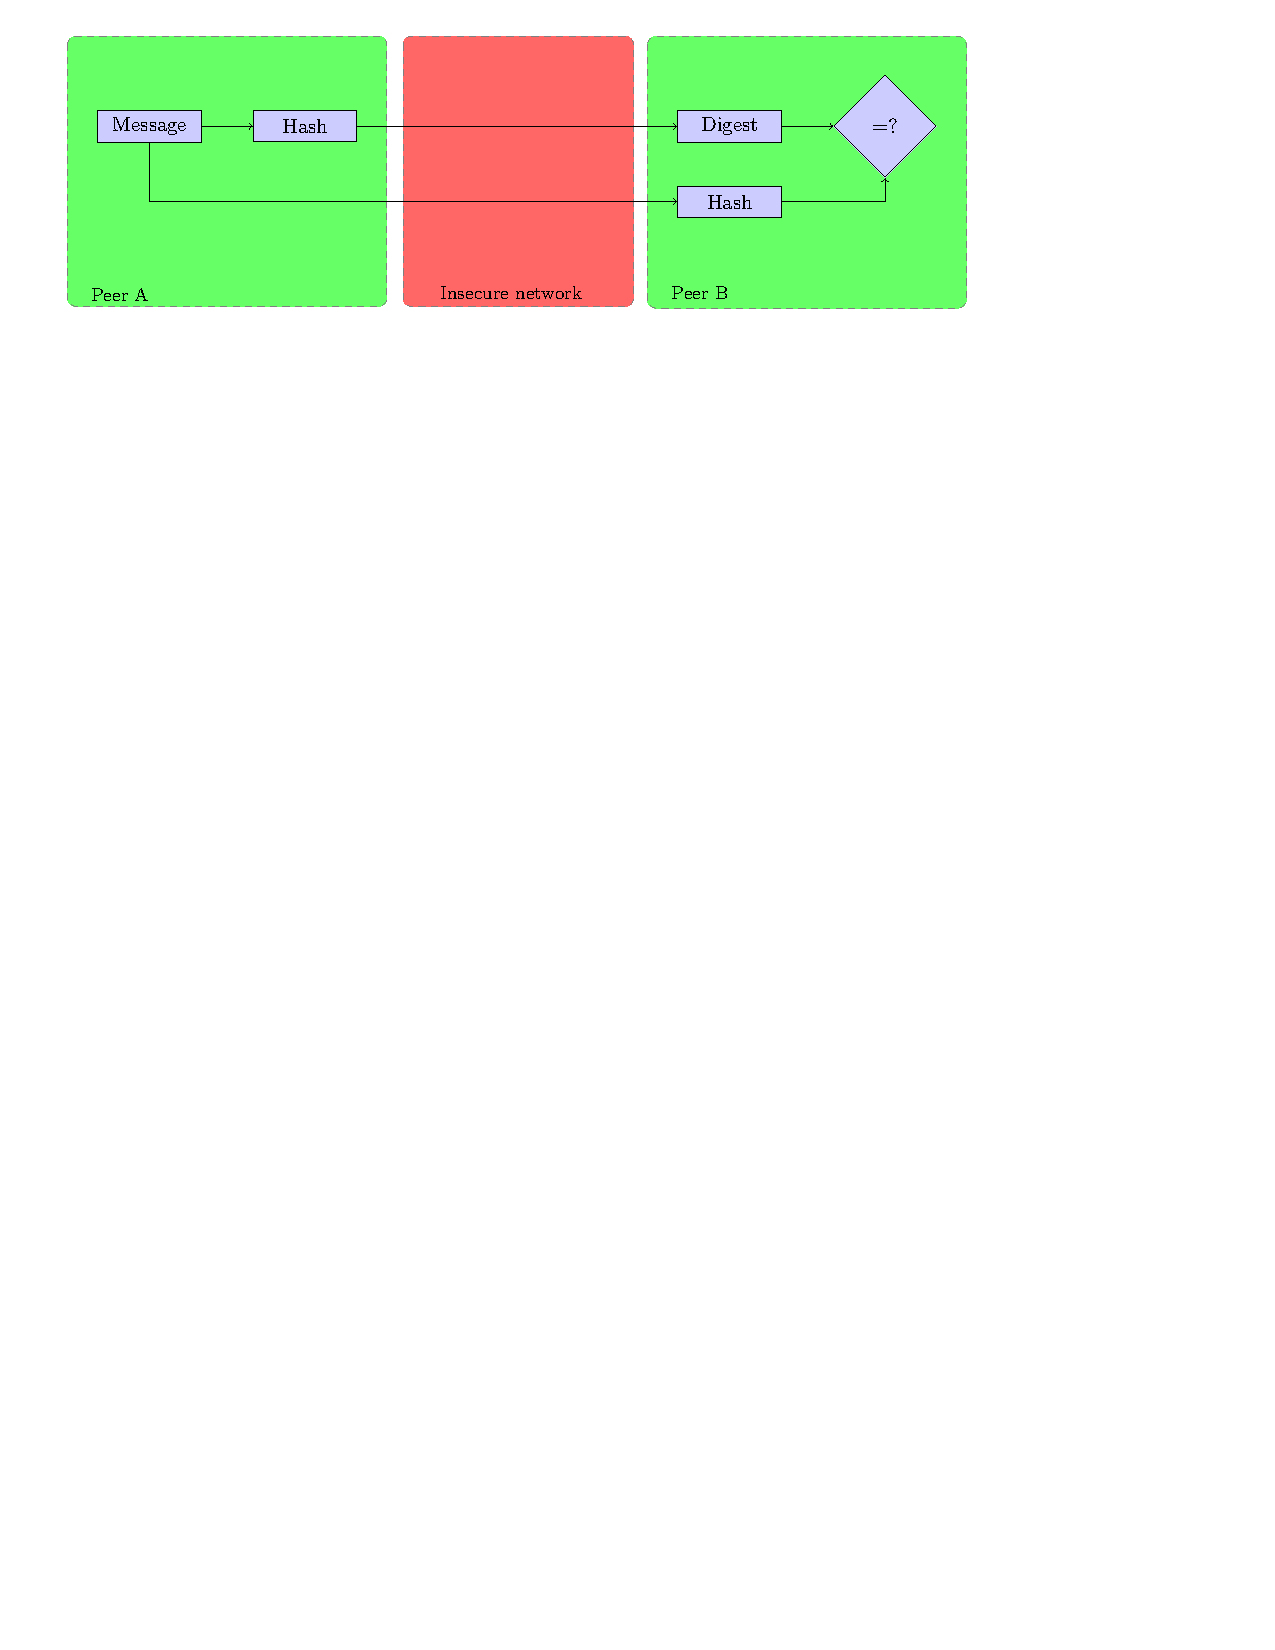
\includegraphics[trim=3.5cm 22.5cm 7.cm 0cm]{figures/hash.pdf}
\caption{Introduction of a hash operation\newline}
\label{fig:hash}
%}
\end{figure}
A cryptographic algorithm is considered practically impossible to invert, meaning
that impossible to recreate the input data (message) with the digest (output of
the hash).
The main properties of a hash function are:
\begin{itemize}
  \item it's quick to compute the digest for any message
  \item it's infeasible to generate a message from its digest
  \item it is infeasible to modify a message without changing the digest
  \item it is infeasible to find two different messages with the same
  digest.\newline
\end{itemize}
On Figure \ref{fig:hash}, the message is hashed and the result (digest) is
sent to the other peer with the original message.\newline Then the other peer
hashes the message too (with the same algorithm) and compares the two digests to
know if the message has been changed during the transmission.\newline 
This is the principle of integrity.

\todo[inline]{Add table with example of hash with same word but one with
capital letter at the beginning (to show the difference)}

\newpage

\subsection{Signature algorithm}
\label{intro_sign}
\begin{figure}[!ht]
\centering
%\frame{
% trim: left, bottom, right, up
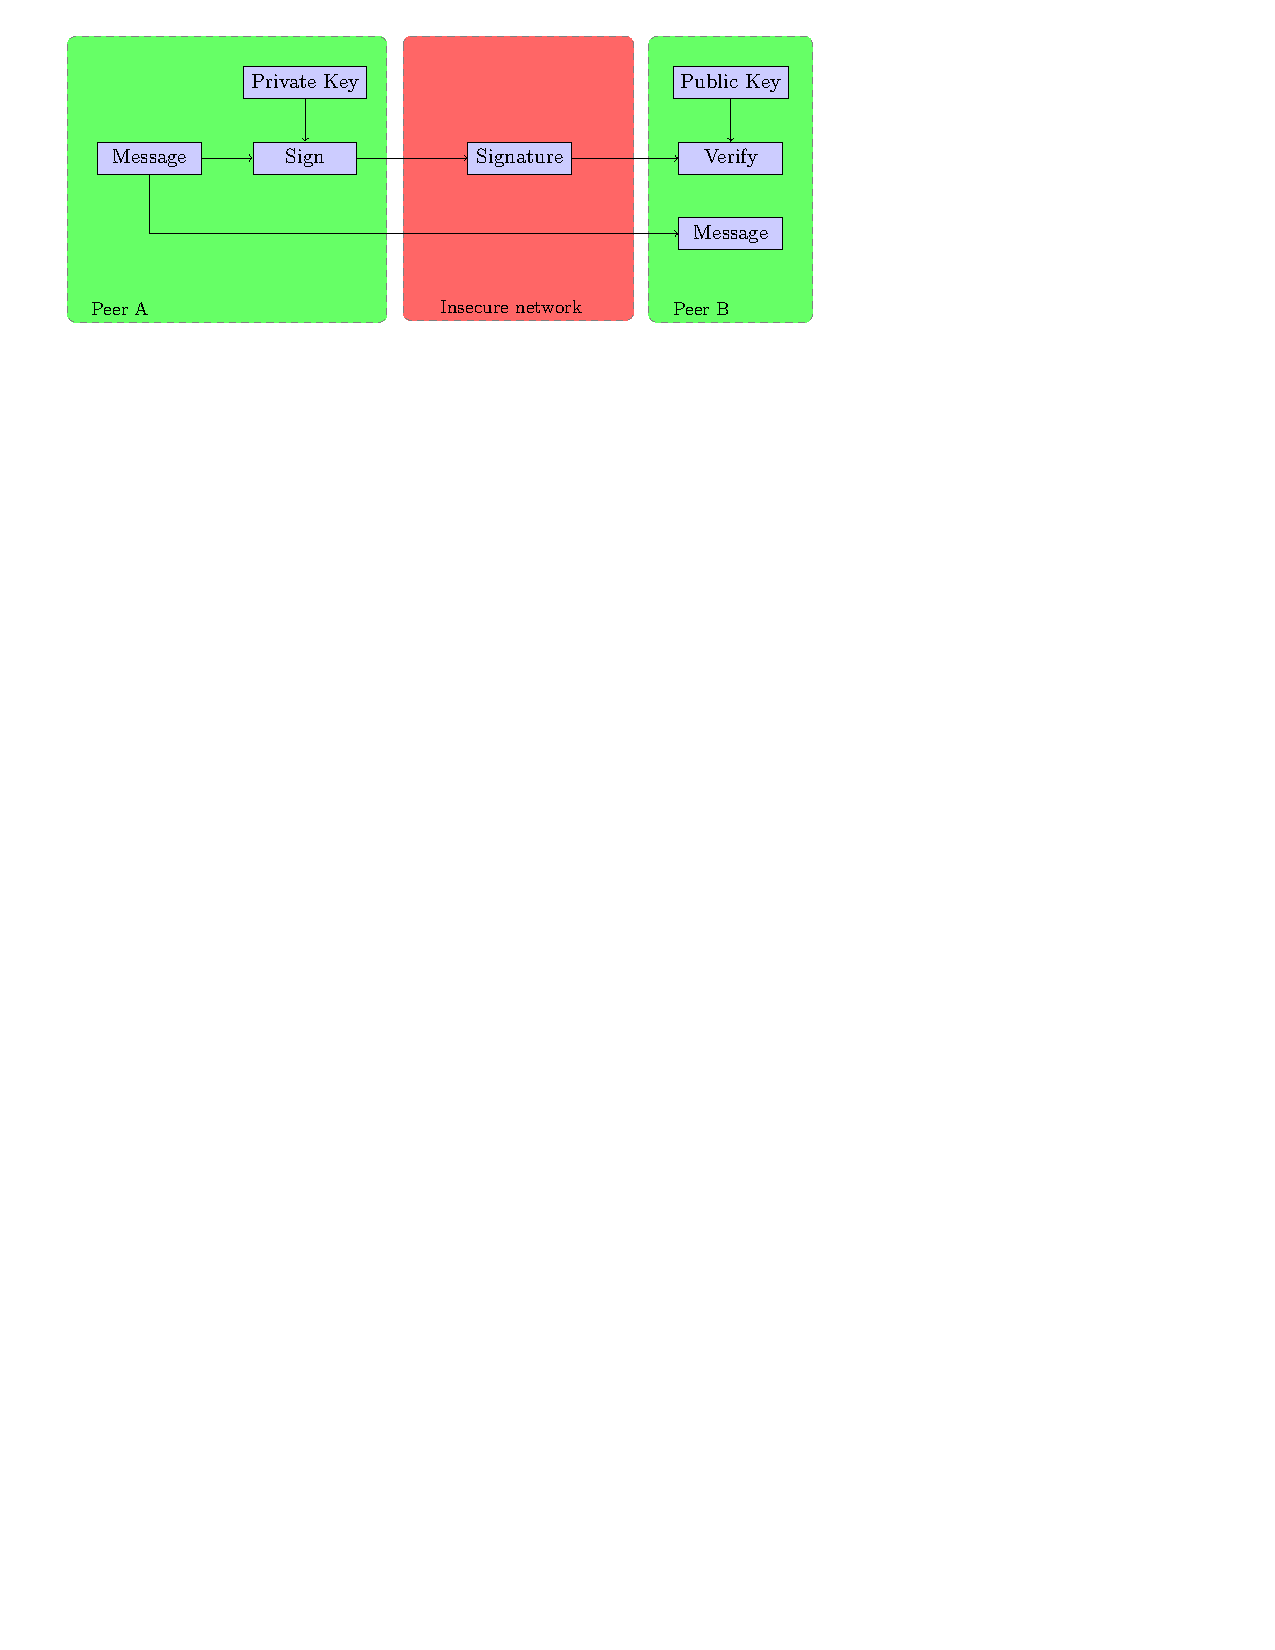
\includegraphics[trim=2cm 22.25cm 7.5cm 0cm]{figures/signature.pdf}
\caption{Introduction of a signature operation\newline}
\label{fig:sign}
%}
\end{figure}
A digital signature is a mathematical principle to demonstrate the authenticity of
a message.\newline

It infeasible to generate the original message with the signature.
A valid digital signature allows to be sure that the incoming message comes from
the peer we are communicated with and not from someone else
(authenticity).\newline
With digital signatures the sender cannot deny having sent the message
(non-repudiation).\newline
It allows too to be sure that the message has not been corrupted during the
transmission (integrity).\newline

The principle of a digital signature is shown figure \ref{fig:sign}.\newline
The message is signed with the private key (no one has this key too) and the
result (signature) is sent to the other peer (peer B).\newline
The public key of the peer A has already been sent previously. With this key, peer
B can verify the signature (only with the public key of peer A) and be sure that
the message sends with it comes from peer A and not from someone else.

\newpage

\subsection{Cipher}
 The cipher is an algorithm uses for encryption of data (plaintext) and
 decryption of data (ciphertext).\newline
 It's uses on internet, on the e-mail, on cellphone when calling, etc.\newline
 Two main cipher algorithms exists, which are:
 \begin{itemize}
   \item Symmetric
   \item Asymmetric
 \end{itemize}



\subsubsection{Symmetric cipher algorithm}
\label{intro_cipher}


Symmetric-key algorithms are algorithms for cryptography that use the same
cryptographic keys for both encryption of plaintext and decryption of
ciphertext in a communication.\newline
The key is often named shared secret key.\newline
There are two kinds of symmetric encryption:
\begin{enumerate}
  \item Stream ciphers, which encrypts bits individually
  \item Block ciphers, which encrypts an entire block of plaintext bits
  at a time with the same key\newline
\end{enumerate}


\begin{figure}[!ht]
\centering
%\frame{
% trim: left, bottom, right, up
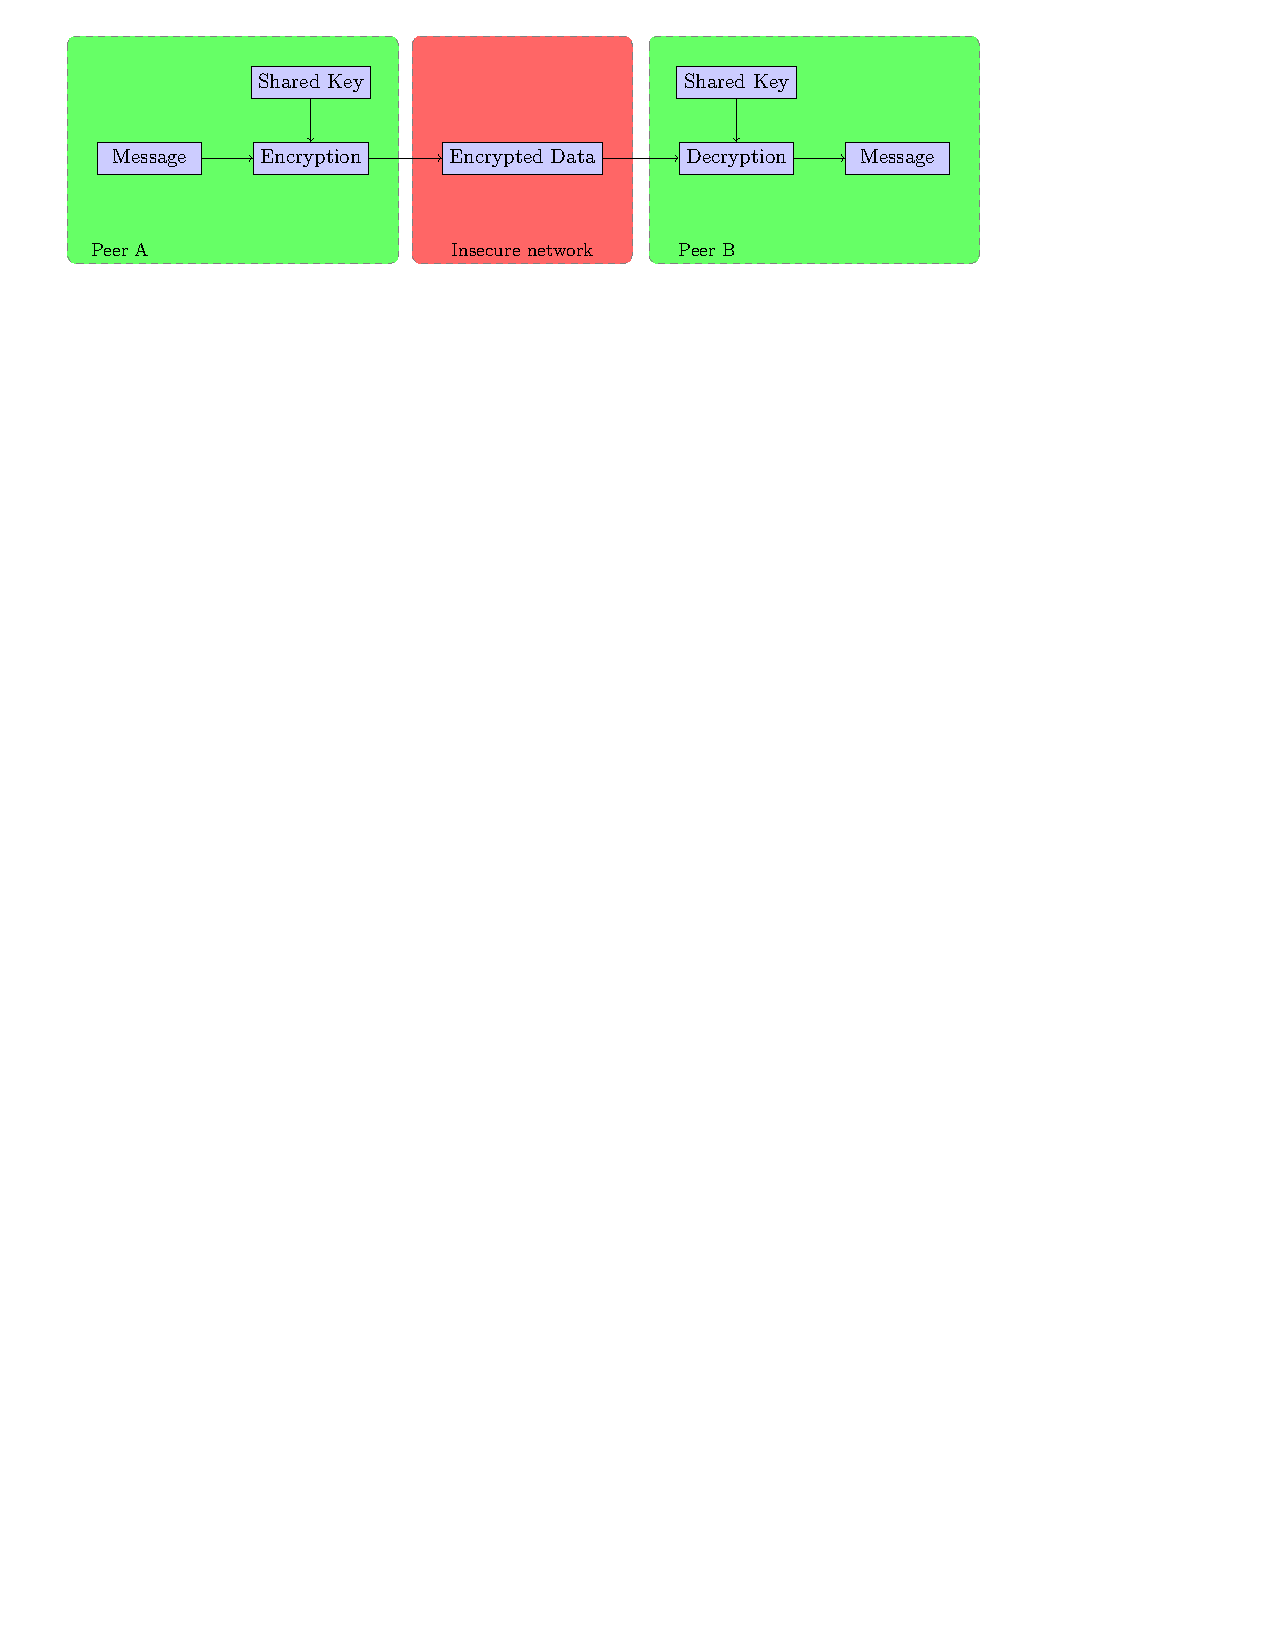
\includegraphics[trim=1cm 23.25cm 4cm 0cm]{figures/sym_cipher.pdf}
\caption{Introduction of a symmetric cipher operation}
\label{fig:sym}

%}
\end{figure}

Figure \ref{fig:sym} represents the process for encryption and decryption with a
symmetric key.
The shared key has already been exchanged between the two peers.\newline
Peer A encrypts the message (plaintext) with this key and sends the result (the
encrypted data or ciphertext) to peer B.\newline
Then peer B uses the same key but to decrypt the encrypted data (ciphertext) and
then reads the plaintext sent by the peer A.\newline

No one who doesn't have this key can understand this message over the insecure
network represents in red figure \ref{fig:sym}.

\newpage
\subsubsection{Asymmetric cipher algorithm}
\label{intro_asym_cipher}

\begin{figure}[!ht]
\centering
%\frame{
% trim: left, bottom, right, up
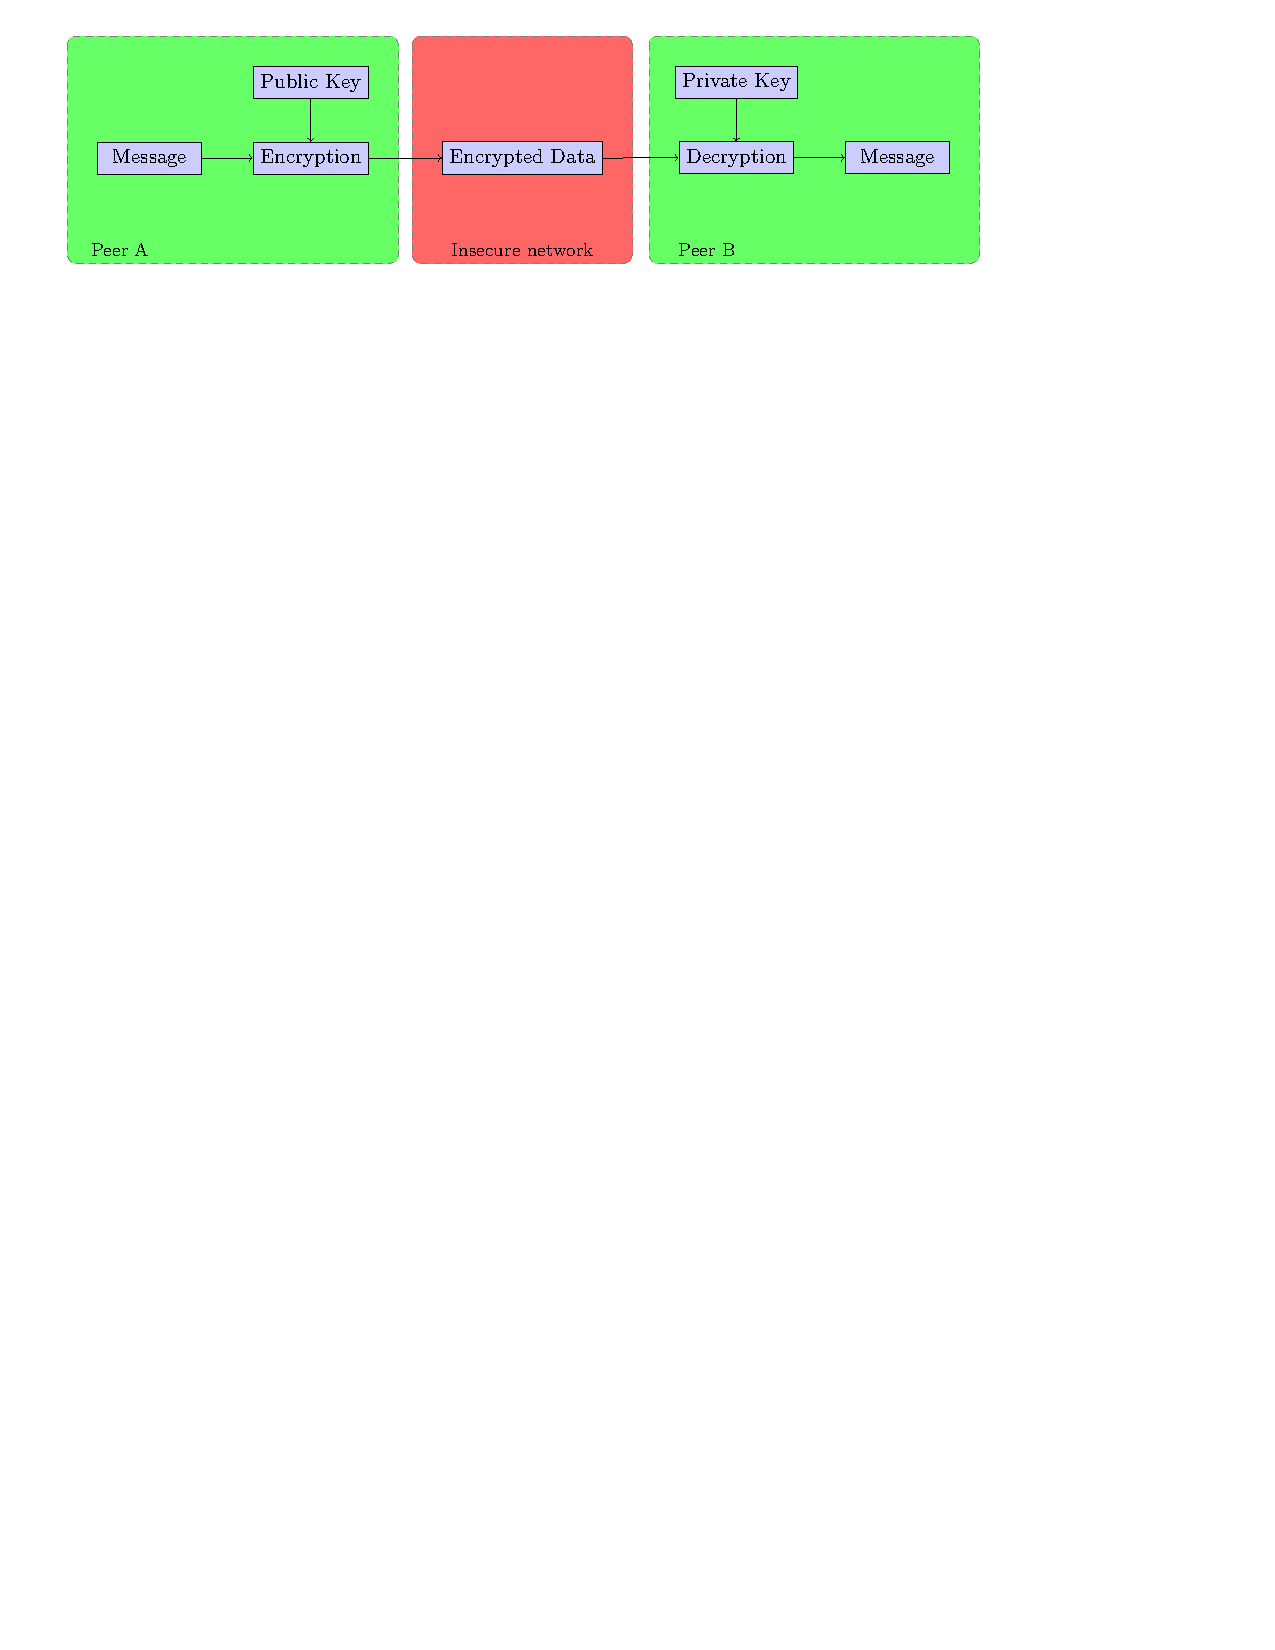
\includegraphics[trim=1cm 23.25cm 4cm 0cm]{figures/asym_cipher.pdf}
\caption{Introduction of an asymmetric cipher operation}
\label{fig:asym}
%}
\end{figure}
Asymmetric algorithm is a method for encryption and decryption of messages with
public and private keys. \newline
One peer generates the private and public key together, keep the private key
(meaning that he is the only one to have it) and sends the public key to every
one he wants to communicate with.\newline
With the public key everyone can encrypt a message, which no one can understand
through the insecure network and no one can decrypt it, except this one who has
the private key.\newline

Figure \ref{fig:asym} shows the principle of encryption and decryption with
asymmetric algorithms.\newline
Peer B is this one that has generated the public and private keys and has already
sent the public key to peer A.\newline
Peer A encrypts the message with the public key of peer B. This
message is than sends to peer B over the insecure network.\newline
Thanks to the private key can peer B decrypts the message of peer A.\newline

Through the principle of private and public keys, asymmetric algorithm allows
privacy (like symmetric algorithm) but integrity of data too, because only this
one who creates the keys has the private key for decryption.

\newpage
\subsection{Diffie-Hellman}
\label{intro_dh}
\begin{figure}[!ht]
\centering
%\frame{
% trim: left, bottom, right, up
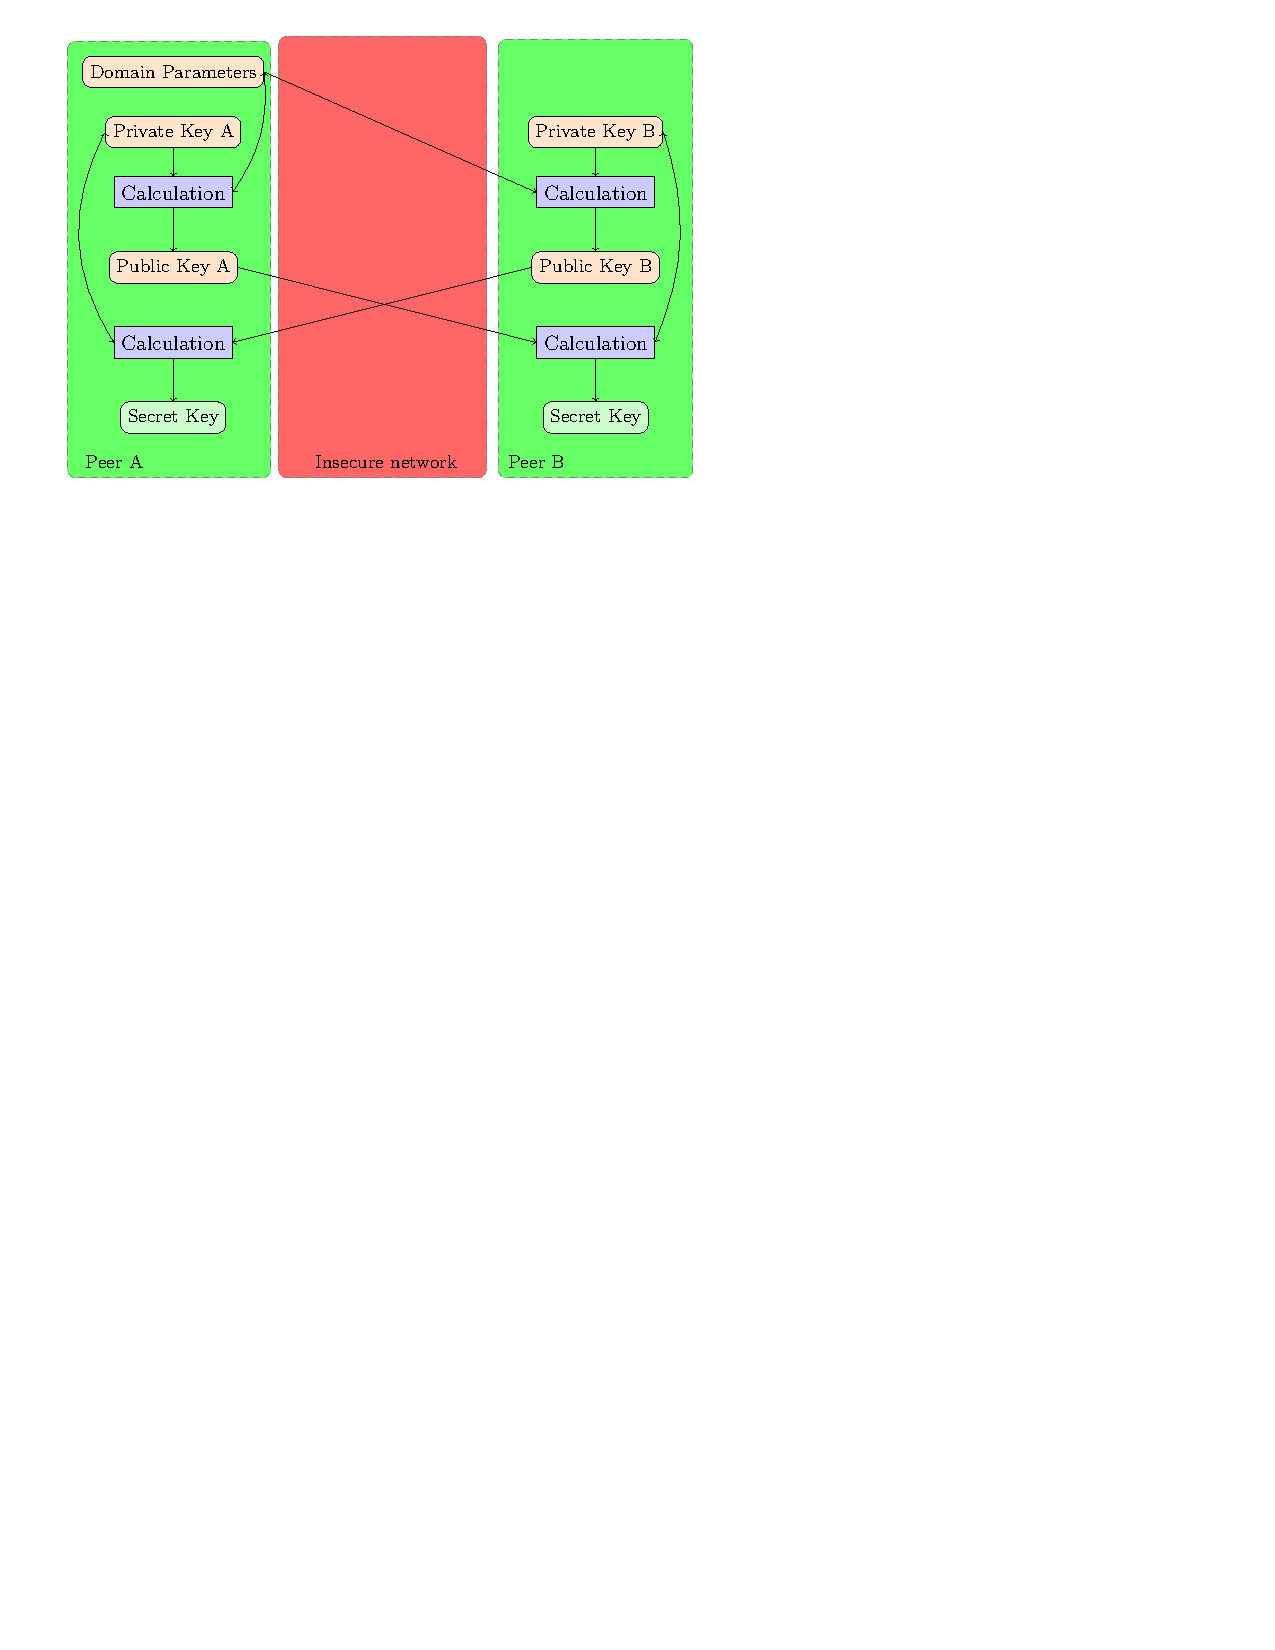
\includegraphics[trim=0cm 20cm 8cm 0cm]{figures/diffie_hellman.pdf}
\caption{Introduction of a Diffie-Hellman operation}
\label{fig:dh}
%}
\end{figure}
Diffie-Hellman Key Exchange establishes a shared secret key between two peers
that can be used for secret communication for exchanging data over an insecure
network.\newline
The principle of Diffie-Hellman Key Exchange is to begin with asymmetric keys and
to finish with symmetric key. \newline
It makes sure that both parties
participate in the generation of the symmetric key.\newline

Figure \ref{fig:dh} shows the principle of the Diffie-Hellman key
exchanges.\newline 
Peer A creates the domain parameters and a private key only (not the
public).\newline With the domain parameters and the private key can peer A
calculates his public key.\newline
He sends than the domain parameters and his public key to peer B.\newline
Peer B generates a private key too and calculates his public key with the domain
parameters from peer A and its own private key.\newline
Peer B sends than his public key to peer A.\newline
To finish, each one calculates the shared secret (which is the same for the
twice) with the public key of the other peer and it's own private key.\newline

The shared secret is the same for the two peers and can be used for encryption
and decryption.
\newpage

\section{SSL/TLS protocol} %around 1/2 pages 
\label{intro_tls}
\begin{figure}[!ht]
\centering
%\frame{
% trim: left, bottom, right, up
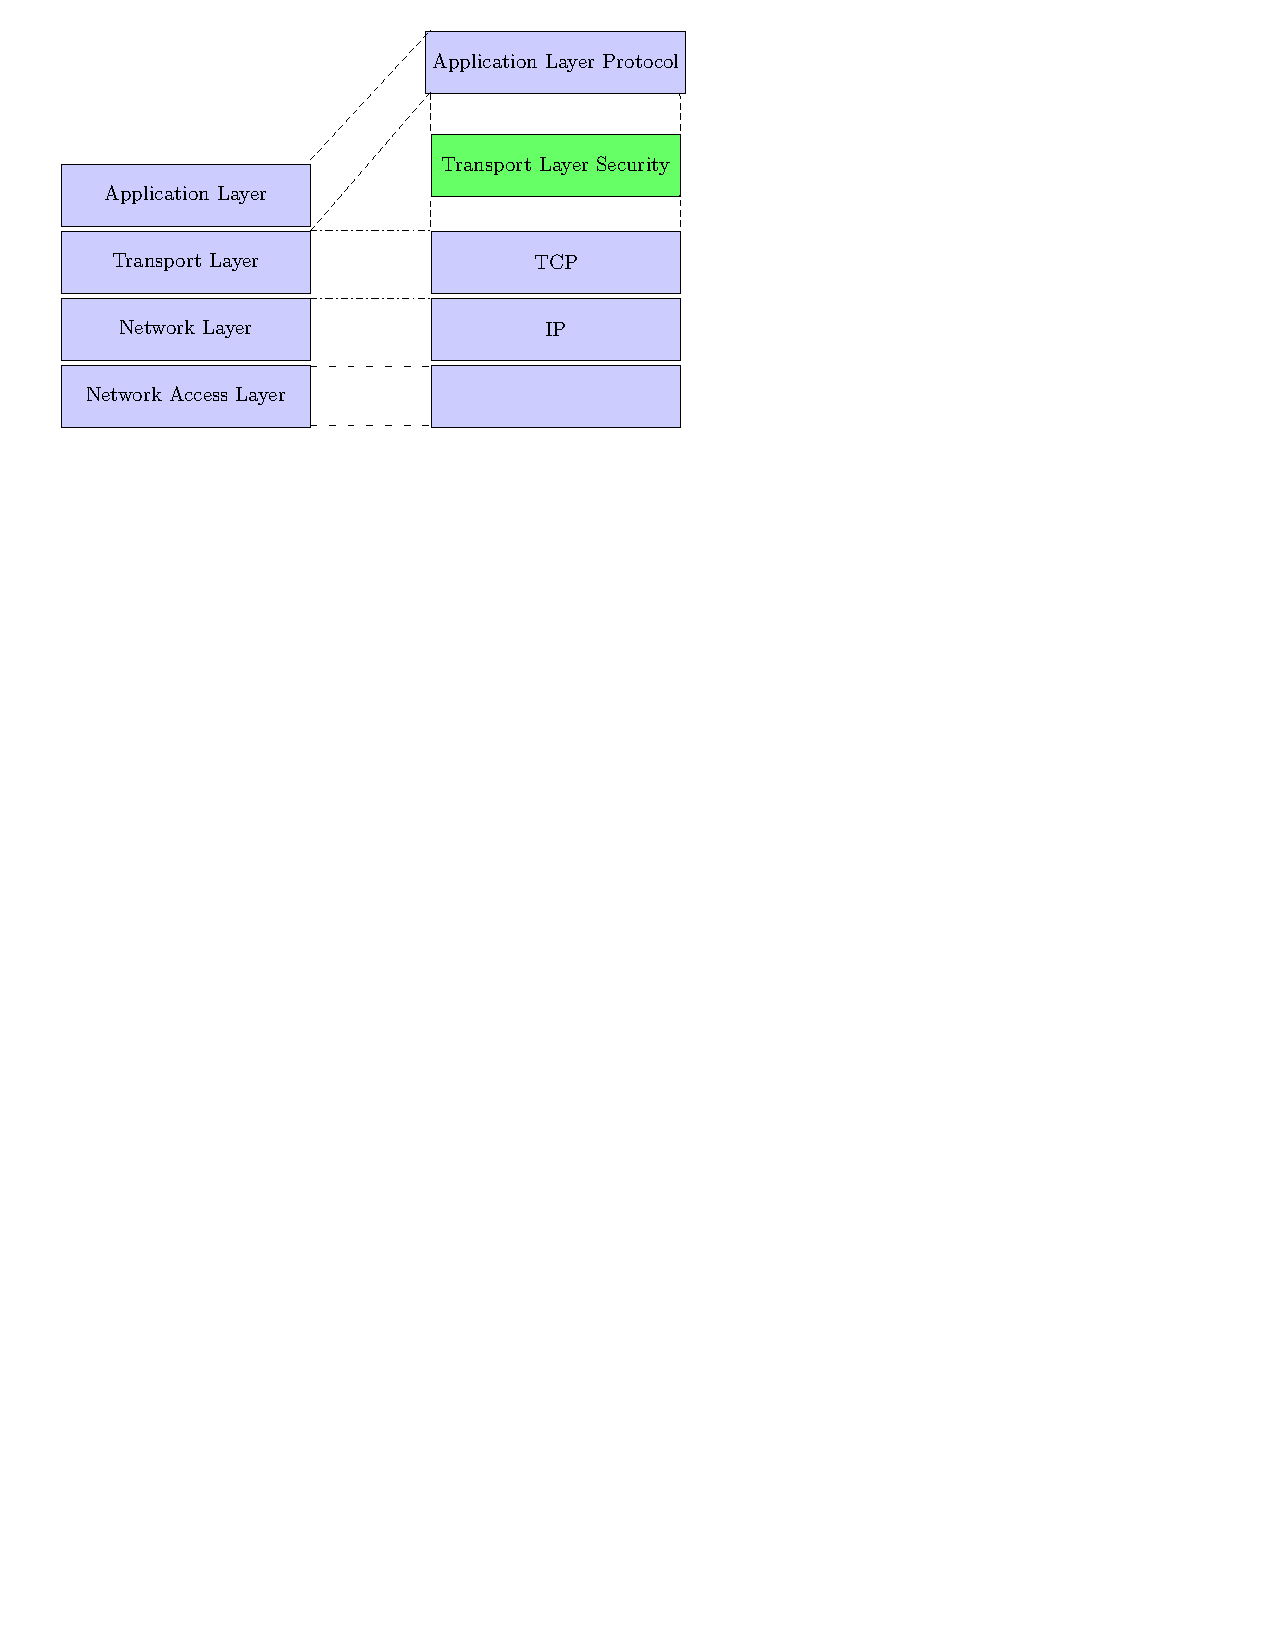
\includegraphics[trim=0cm 20cm 8cm 0cm]{figures/tls_osi.pdf}
\caption{TLS protocol in OSI model}
\label{fig:osi}
%}
\end{figure}
Transport Layer Security (TLS) is a client/server protocol that provides
different basic security services for the communication between peers:
\begin{itemize}
  \item Authentication (both peer and data origin authentication)
  services
  \item Connection confidentiality services
  \item Connection integrity services (without recovery)
\end{itemize}
This security layer is situated between the transport and the application layer
on the OSI model (see figure \ref{fig:osi})
This security protocol is often uses in:
\begin{itemize}
  \item E-commerce website for secured transaction and client authentication
  access
  \item Remote access
  \item Web browsers to browse the Internet
  \item Simple Mail Transfer Protocol (SMTP)
  \item Virtual Private Network (VPN)
\end{itemize}

\subsection{Handshake protocol}

\todo[inline]{Explain Handshake protocol}

\subsubsection*{Client Hello}

\subsubsection*{Server Hello}

\subsubsection*{ChangeCipherSpec}

\subsubsection*{Application Data}
